\section{评估}
\label{sec:evaluation}

本节从内核级与端到端两个层面对 \sys v0.2 进行评估，展示其设计如何应对 LLM 服务中的关键挑战。结果表明：在 LLM 服务基准中，相比 Triton 后端，\sys 可将 token 间时延降低 29-69\%；在长上下文推理中可降低 28-30\% 时延；在并行生成中可获得 13-17\% 加速。实验在 NVIDIA A100 40GB SXM 与 H100 80GB SXM 上进行，使用 CUDA 12.4、PyTorch 2.4.0，存储与计算精度为 f16。

\subsection{端到端 LLM 服务性能}

我们在 SGLang v0.3.4~\cite{zheng2023sglang} 上评估 \sys，并与 SGLang + Triton v3.0~\cite{triton} 对比。后者是面向 NVIDIA GPU 的领先 LLM 服务引擎，但其注意力内核闭源，限制了透明性与社区优化潜力。为保证评估全面性，我们使用两类数据集：常用 ShareGPT 数据集\footnote{\url{https://huggingface.co/datasets/anon8231489123/ShareGPT_Vicuna_unfiltered/resolve/main/ShareGPT_V3_unfiltered_cleaned_split.json}} 与合成负载（Variable，序列长度在 512 到 2048 间均匀分布）。我们在时延敏感在线服务设置下测量 TTFT（time-to-first-token）与 ITL（inter-token-latency），并调整请求率使 P99 TTFT 保持在 200ms 以下。

\begin{figure}[ht]
    \centering
    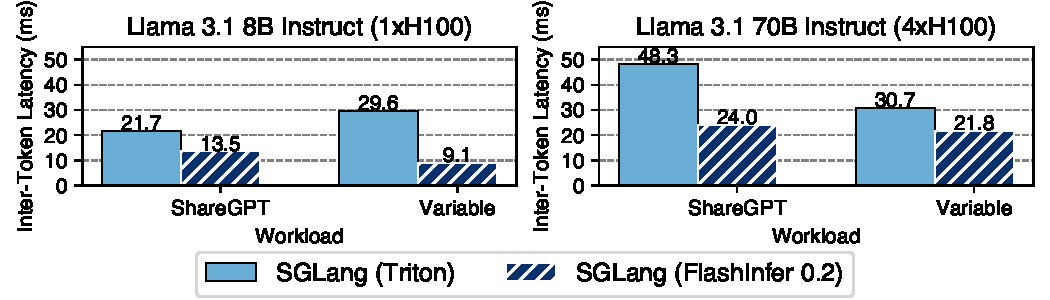
\includegraphics[width=0.45\textwidth]{figures/sglang-itl.pdf}
    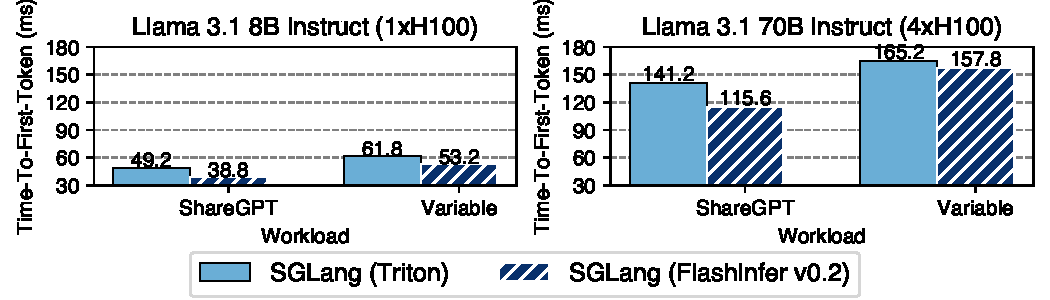
\includegraphics[width=0.45\textwidth]{figures/sglang-ttft.pdf}
    \caption{集成 \sys 与 Triton 的 SGLang 的中位 ITL 与中位 TTFT。}
    \label{fig:sglang-itl-ttft}
\end{figure}

图 \ref{fig:sglang-itl-ttft} 展示了在 Llama 3.1 8B（1xH100）与 Llama 3.1 70B（4xH100）上的 ITL 与 TTFT。相较 Triton 后端，\sys 后端在所有设置下都表现出稳定加速。

\subsection{输入动态性下的内核性能}
\label{eval:input-dynamism}

本节在不同序列长度分布下，对比 \sys 生成内核与开源 SOTA FlashAttention 库性能。我们使用其最新主分支\footnote{Commit: \href{https://github.com/Dao-AILab/flash-attention/commit/c1d146cbd5becd9e33634b1310c2d27a49c7e862}{c1d146c}}（包含 FlashAttention2 与 FlashAttention3）。固定 batch size 为 16，并测试三种长度分布：常数（1024）、均匀分布（512 到 1024）与偏斜分布（均值 1024 的 Zipf）。prefill 内核启用因果掩码，这是 LLM 服务的常见设置。

\begin{figure}[ht]
    \centering
    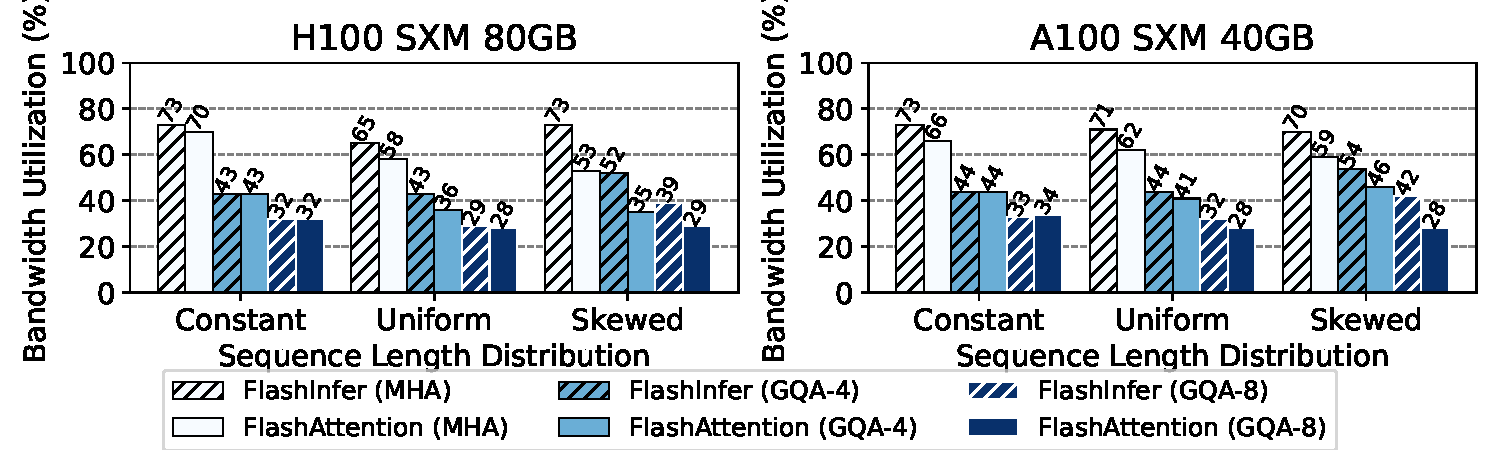
\includegraphics[width=0.45\textwidth]{figures/varlen-decode.pdf}
    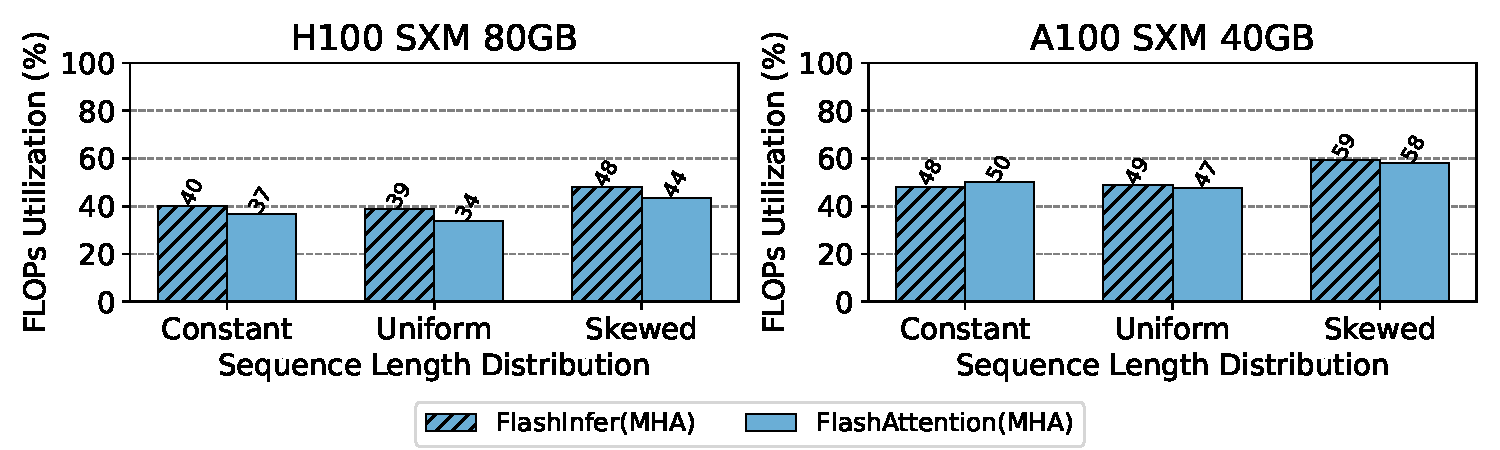
\includegraphics[width=0.45\textwidth]{figures/varlen-prefill.pdf}
    \caption{decode（上）与 prefill（下）内核的带宽利用率与 FLOPs 利用率（越高越好）。}
    \label{fig:varlen}
\end{figure}

图 \ref{fig:varlen} 给出了 decode 与 prefill 内核的带宽/FLOPs 利用率。由于我们的动态负载均衡调度器（第 \ref{sec:load-balanced-scheduling} 节），\sys 在均匀与偏斜长度分布下显著优于 FlashAttention。\sys 在 decode 场景也优于 FlashAttention，原因在于我们支持更灵活的 tile 大小选择（第 \ref{sec:tile-size-selection} 节），而 FlashAttention 在解码场景使用了次优 tile 配置。

\subsection{面向长上下文推理的可定制性}

本节展示 \sys 的定制化注意力内核如何显著加速 LLM 推理。我们关注 Streaming-LLM~\cite{xiao2023streamingllm}，该算法可在常量 GPU 内存下实现百万 token 推理。Streaming-LLM 对专用注意力内核有较强需求，特别是 RoPE~\cite{su2024rope} 与注意力融合内核；\sys 仅需额外约 20 行 query/key 变换代码即可生成此类融合内核。我们对比 \sys 融合内核与非融合内核（\sys 与 FlashAttention），并量化 \sys 集成后端到端时延收益。
\begin{figure}[ht]
    \centering
    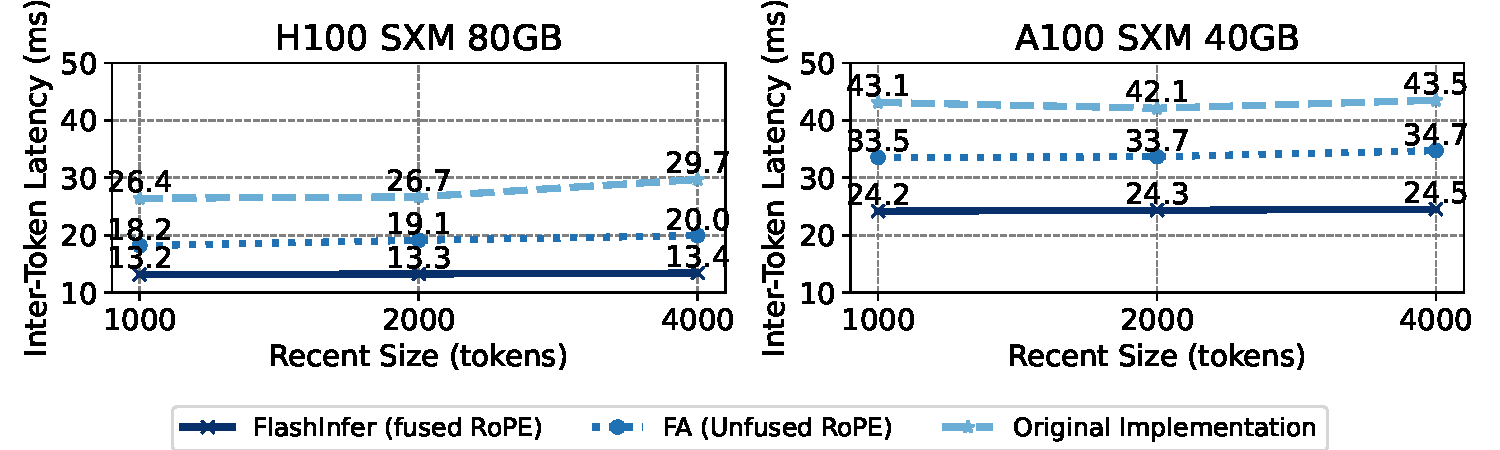
\includegraphics[width=0.4\textwidth]{figures/streaming-llm.pdf}
    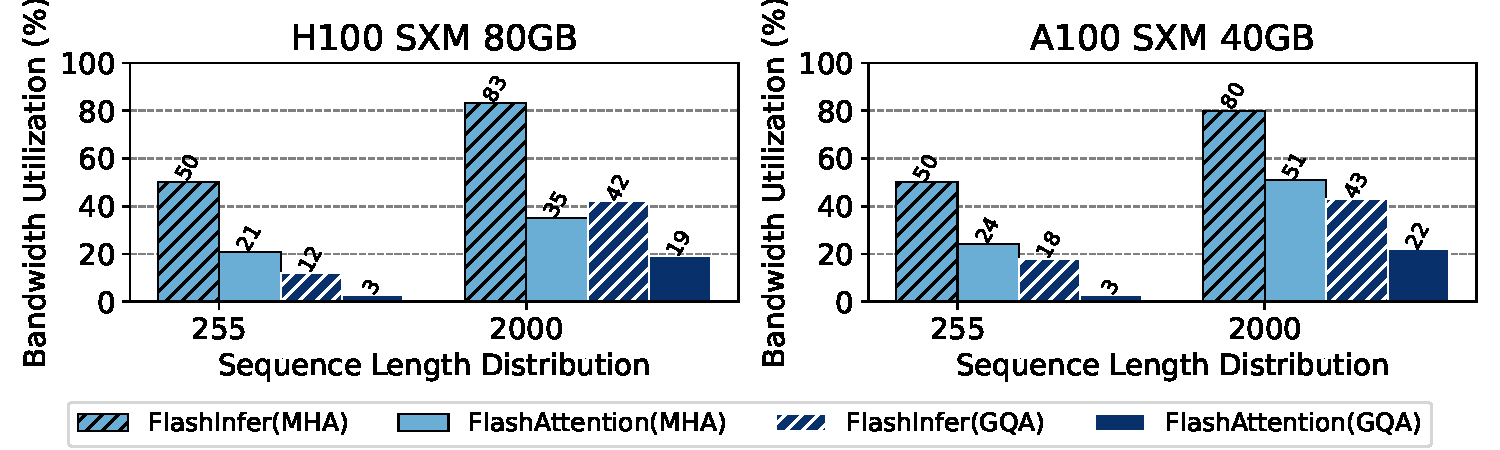
\includegraphics[width=0.4\textwidth]{figures/fused-rope.pdf}
    \caption{上：Streaming-LLM 使用 \sys 融合内核与 FlashAttention 非融合内核的端到端时延（含原始实现）。下：\sys 融合 RoPE 内核相对 FlashAttention 非融合内核的带宽利用率。}
    \label{fig:streaming-llm}
\end{figure}

端到端实验中，我们在 MT-Bench~\cite{zhenbg2023mtbench} 上运行 Vicuna-13B~\cite{vicuna2023} 推理，并测量启用/禁用 \sys 内核时的 ITL。图 \ref{fig:streaming-llm} 显示，在我们优化后的 Streaming-LLM 实现中（原实现存在额外开销），\sys 融合内核在不同配置（通过改变 recent window size）下可带来 28-30\% 的时延下降。我们同时给出 \sys 融合 RoPE 内核与“FlashAttention 的 RoPE + FlashAttention 注意力”组合的内核级对比。\sys 融合内核的带宽利用率提升达 1.6-3.7x，说明可定制注意力内核非常关键。

\subsection{并行生成性能}
\label{eval:memory-heterogeneity}

本节说明 \sys 的可组合格式如何提升并行解码。并行生成已成为 LLM 服务的重要任务，在 LLM agent 场景中尤为有用。OpenAI API 通过 \texttt{"n"} 参数\footnote{\url{https://platform.openai.com/docs/api-reference/chat/create}} 支持一次生成多个候选。由于常存在共享前缀，prefix-caching 可显著提升并行生成效率。\sys 的可组合格式（第 \ref{sec:composable-formats} 节）可将共享前缀与后缀的注意力计算解耦，从而加速并行解码。
\begin{figure}[ht]
\centering
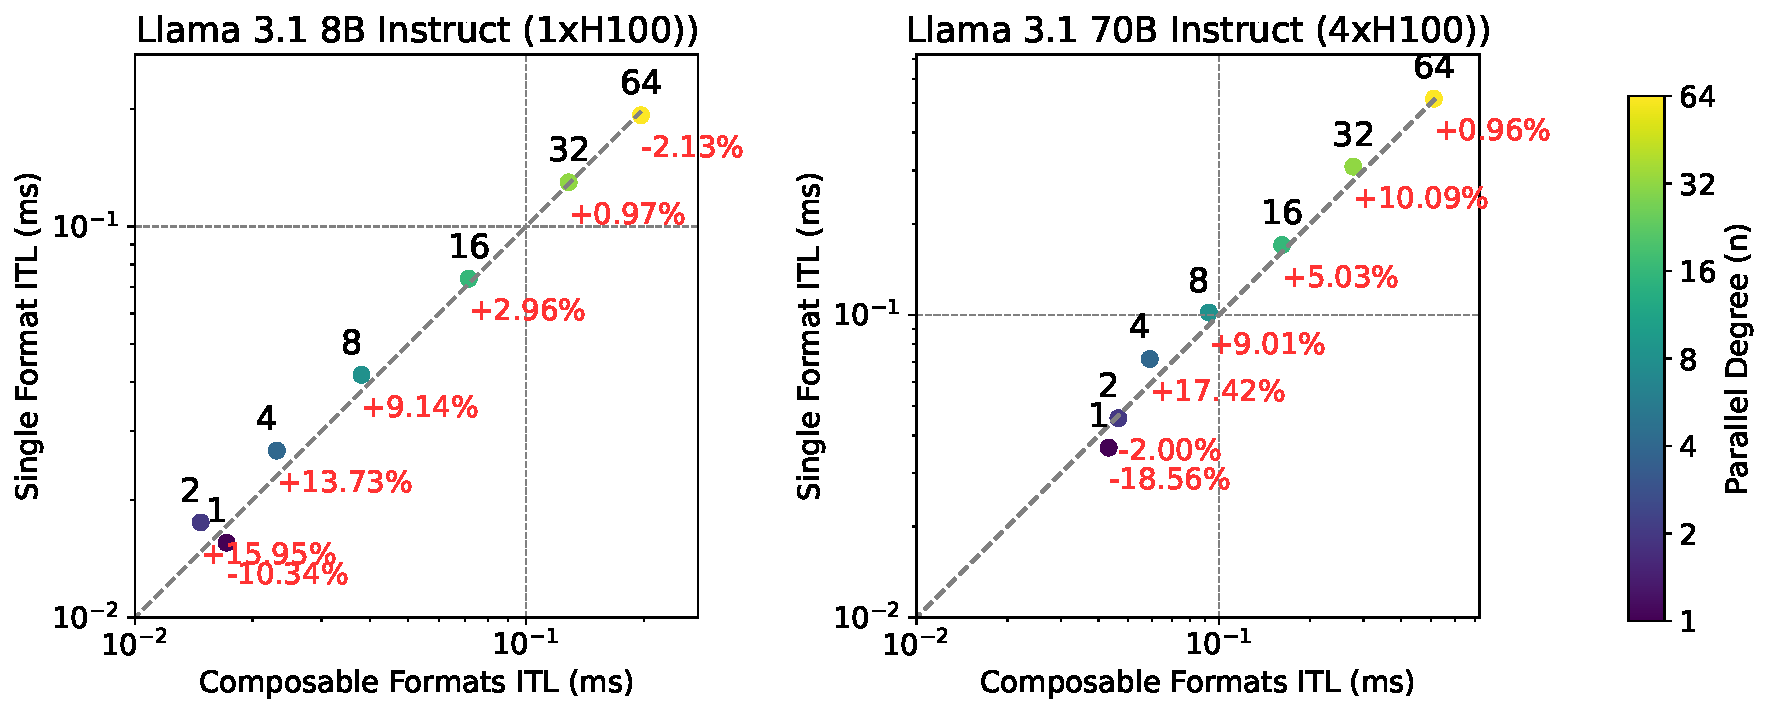
\includegraphics[width=0.4\textwidth]{figures/paragen-itl.pdf}
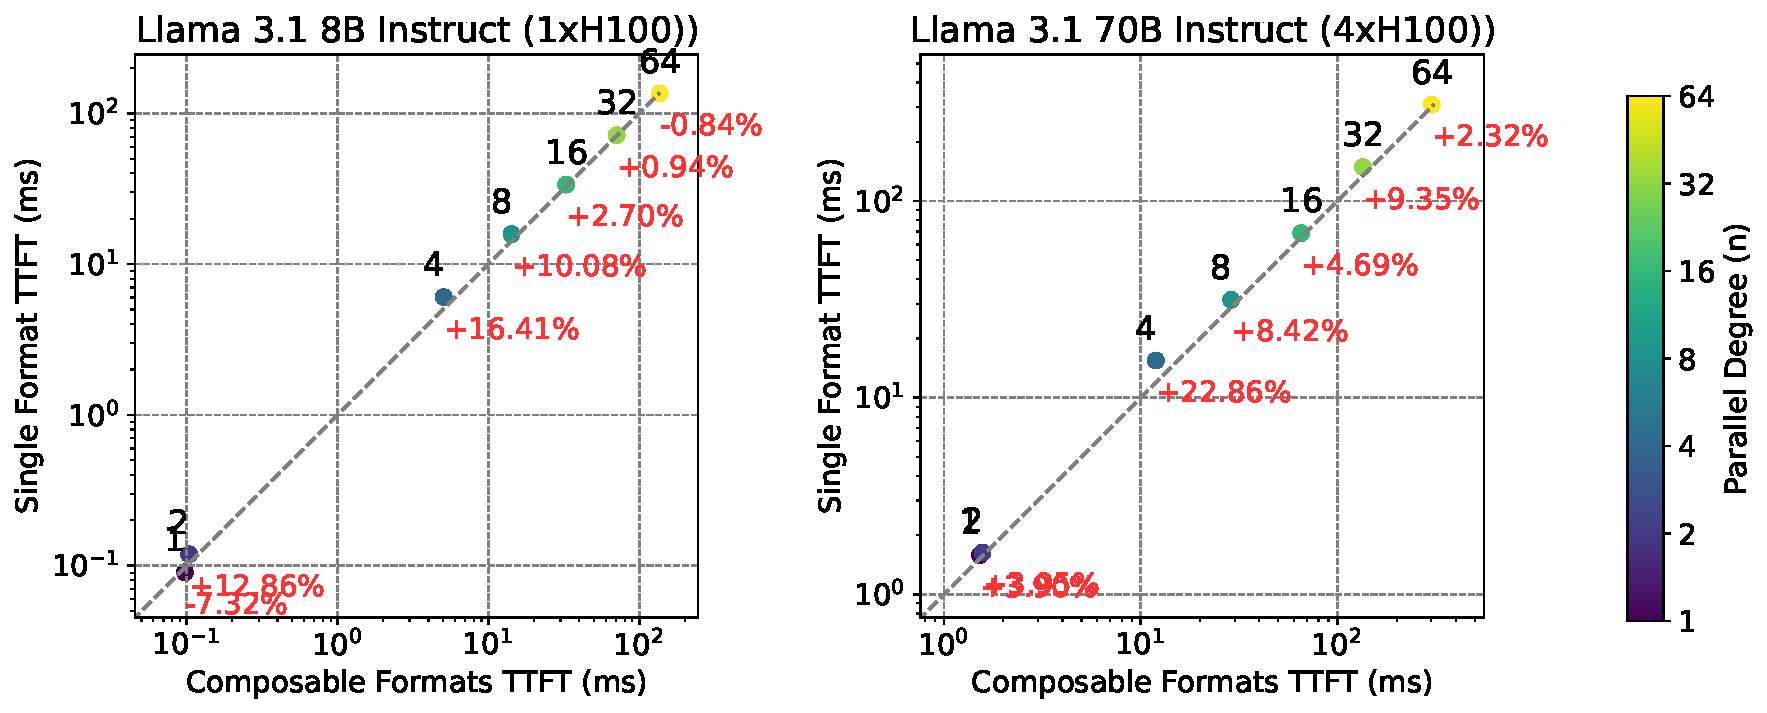
\includegraphics[width=0.4\textwidth]{figures/paragen-ttft.pdf}
\caption{MLC-Engine 在并行生成下启用/禁用可组合格式的 ITL 与 TTFT。横轴表示可组合格式性能，纵轴表示单格式性能；点在对角线上方表示可组合格式更优。不同颜色对应不同并行生成 $n$。}
\label{fig:parallel-generation}
\end{figure}

我们在启用 prefix-caching 的 MLC-Engine~\cite{mlcllm} 中实现可组合格式，并评估并行生成性能。实验使用 Llama 3.1 8B/70B~\cite{llama31} 与 ShareGPT，固定请求率为 16，并将并行 token 数设置为 $\{1,2,4,8,16,32,64\}$，对比关闭可组合格式的配置。图 \ref{fig:parallel-generation} 给出了启用/禁用可组合格式时的 ITL 与 TTFT。

在中等并行度（$4 \leq n \leq 32$）下，\sys 的可组合格式在 ITL 与 TTFT 上均带来稳定加速。峰值出现在 $n=4$：8B/70B 的 ITL 分别下降 $13.73\%$/$17.42\%$，TTFT 分别下降 $16.41\%$/$22.86\%$。较小 $n$ 下，由于块大小提升不足，收益有限；较大 $n$ 下，计算不再主要由注意力主导（尤其 ShareGPT 序列较短），可组合格式优势趋于平台期。
